\documentclass[a4paper,10pt]{article}
\usepackage[utf8]{inputenc}
\usepackage[margin=3cm]{geometry}
\usepackage{amsmath}
\usepackage{amssymb}
\usepackage{amsthm}
\usepackage{fancyhdr}
\usepackage{seminar}
\usepackage{graphicx}
%\usepackage{subfigure}
\usepackage{float}
\usepackage{hyperref}
\usepackage{bm}
\usepackage{cleveref}
\usepackage[rightcaption]{sidecap} % side caption
\usepackage{caption}
\usepackage{subcaption} % for two columns figure
\pagestyle{fancy}


%You can add theorem-like environments (e.g. remark, definition, ...) if you want
\newtheorem{theorem}{Theorem}

\title{Seminar Report on Cubic Stylization} % Replace with your title
\author{Meng Liu} % Replace with your name
\institute{Robotics, Cognition, Intelligence\quad\quad Technische Universit\"{a}t M\"{u}nchen} % Replace with the department you belong to

\makeatletter
\let\runauthor\@author
\let\runtitle\@title
\makeatother
\lhead{\runauthor}
\rhead{\runtitle}


\begin{document}

\maketitle

\begin{abstract}
In this report, a paper Cubic Stylization \cite{Liu:CubicStyle:2019} from Hsueh-Ti Derek Liu and Alec Jacobson will be discussed in detail. Published in year 2019, this work proposes a novel algorithm to turn a 3D shape into a style of a cube and preserve the detail of the original shape at the same time. To achieve the goal, as-rigid-as-possible and $\ell$1-norm are introduced to build up the objective function; ADMM (alternating direction method of multipliers) and affine progressive mesh are adapted to solve the optimization problem efficiently. Some sophisticated artistic controls are provided and discussed at the end of this report.

\end{abstract}
 
\section{Introduction}
In computer graphics and interactive design, cubic stylization means convert a 3D object into a shape of a cube. However, this modeling has a quite long history in the art domain. From the exhibition of Fondation Giacometti in Paris to private collection of Tai-chi series statue; from crystal sculpture to wood carving, shown in figure \ref{fig:arts}, this geometric modeling is quite widespread across the world and time.

	\begin{SCfigure}[1][h]
	    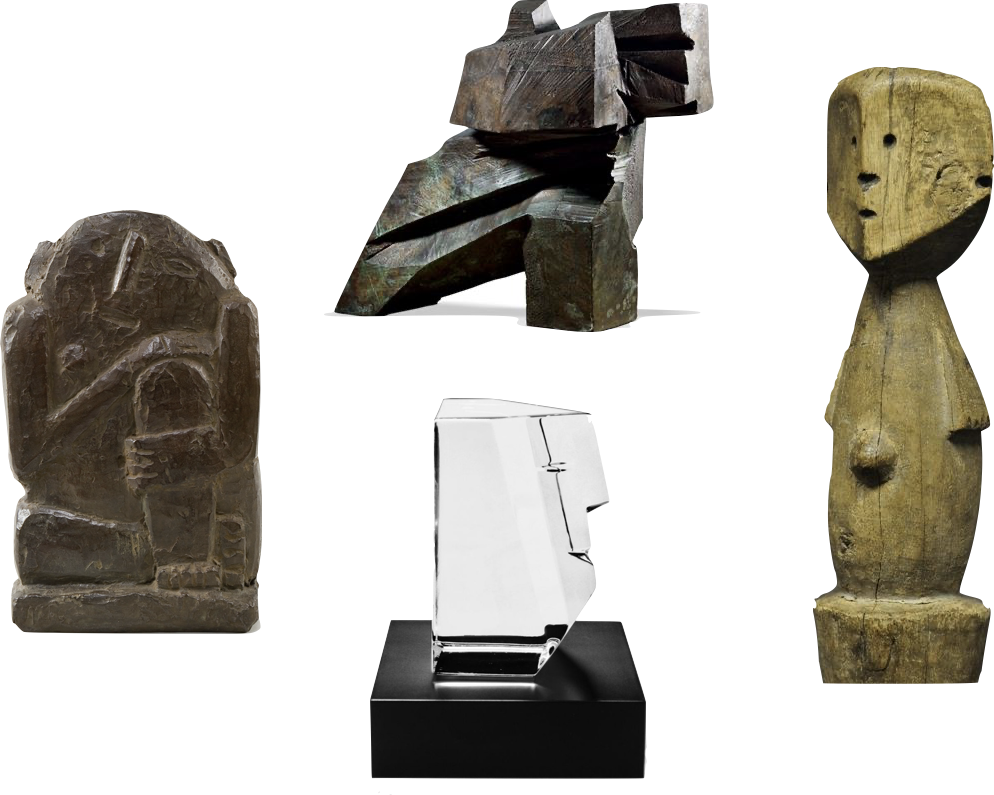
\includegraphics[width=0.45\linewidth]{figures/arts.png}
	    \caption{Alberto Giacometti, Personnage accroupi, Fondation Giacometti, Paris (left). Taichi Series: Thrust, Zhu Ming, private collection (upper middle). Crystal cubic sculpture from an online store Sweden (lower middle). Azande Wood Post, DRC, African Wood Carvings (right).}
	    \label{fig:arts}
	\end{SCfigure}
	
Not only art creation, the need of cubic stylization also come from industrial, e.g. film visual effects. That’s why it is also naturally to think about simulating and speeding up the stylization process with a computer when a non-cubified object at hand. In this report, the core idea and the implementation of the paper \cite{Liu:CubicStyle:2019} will be presented in the following steps:
	\begin{itemize}
		\item two building blocks of the objective function will be introduced in section \ref{norm} and \ref{arap} respectively, 
		\item the update rules of ADMM for solving the optimization problem is derived from scratch in section \ref{admm},
		\item the adaptation of Affine Progressive Method to shorten the computing time is introduced in section \ref{affine},
		\item and some artistic controls which provided by the model to make the stylization more flexible and meet the need of modelers are presented in section \ref{artistic}.
	\end{itemize}

%-----------------------------------------------------------------------------------------------------
% Method description
%-----------------------------------------------------------------------------------------------------
\section{Method description}\label{descrip}
Comparing to previous works, which output a 2D image, this paper focuses on a more general setting. Given a 3D object in the form of triangular mesh, after processing, it should provide a similar 3D object but in cubic shape. Intuitively, we should let as many faces as possible of a triangular mesh orthogonal to one of the axes of the global coordinate. We can use the normals of a triangular mesh to simplify this, which means the normals should be parallel to one of global coordinate axes. These kinds of vector share one of the forms, $(x,0,0)$, $(0,y,0)$ or $(0,0,z)$, in which most of coordinates are zeros expect one. These sparse vectors lead us to the first part of the objective.

%-----------------------------------------------------------------------------------------------------
% Objective Function
%-----------------------------------------------------------------------------------------------------
\subsection{Objective Function}\label{objective}

%-------------------------------------------------------------------
% L1 norm
%-------------------------------------------------------------------
\subsubsection{Sparsity effect of the $\ell$1-norm}\label{norm}
Sparsity effect of $\ell$1-norm has been explored extensively from machine learning, control theory or any other domains which uses optimization. Even though this property has been of benefit to wild range of sciences without doubt, it is also beneficial to ask why $\ell$1-norm leads to sparsity. As we can see from the figure \ref{fig:circle} here. 
	\begin{figure}[ht!]
		\centering
		\begin{minipage}[t]{.45\textwidth}
			  \centering
			  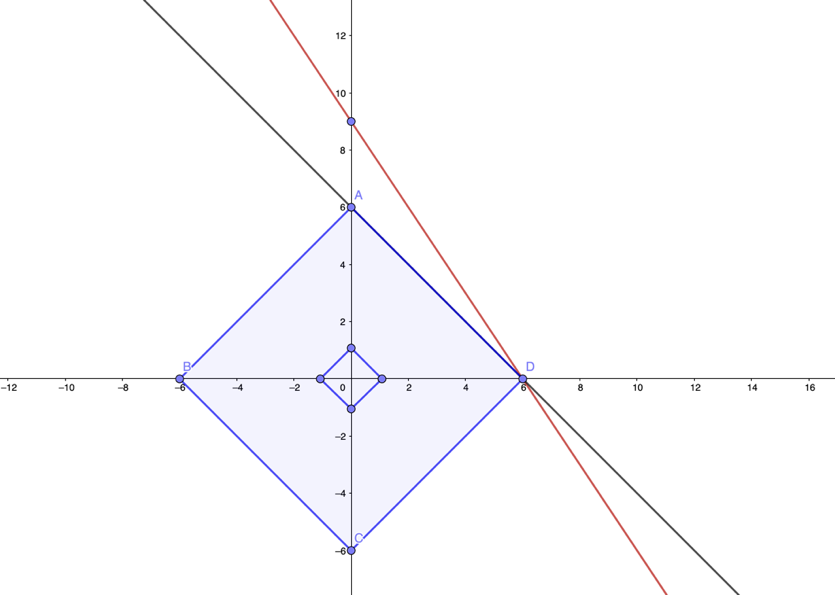
\includegraphics[width=\linewidth]{figures/circle}
			  \captionof{figure}{A set circles of $\ell$1-norm}
			  \label{fig:circle}
		\end{minipage}%
		\begin{minipage}[t]{.55\textwidth}
			  \centering
			  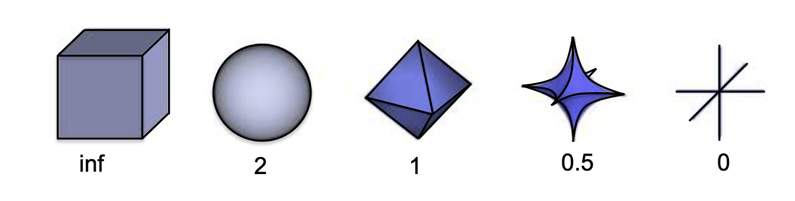
\includegraphics[width=\linewidth]{figures/norms}
			  \captionof{figure}{Unit spheres of different norms\cite{chen:norm}.}
			  \label{fig:norms}
		\end{minipage}
	\end{figure}
Suppose the red line is an object function in 2D plane, we need to find the optimal solution according to $\ell$1-norm. So we first draw the unit circle of the $\ell$1-norm, and gradually enlarge this circle, the first point touches the red line is the optimal point. And normally and mostly, the point is one of the vertices of the circle. This is what we mean by sparsity because one of the coordinate is 0. However, as you can see from the black line case, if the object function has a slope which is parallel to one of the edge of the unit circle, the sparsity effect may not be realized. That is why the correct way to phrase this is that $\ell$1-norm encourages sparsity, but it does not guarantee sparsity. In fact, any $\ell$$p$-norm, with $0\leq p <1$ potentiality gives better sparsity, see figure \ref{fig:norms}, however, they are less deployed due to non-convexity. \\

Back to our problem, after transforming the surface, we enforce normals to align to global coordinate axes. This is defined by the following Cubeness term,
	\begin{equation*}
  		CUBENESS := \sum_{i\in V} \left\lVert R_i \hat{n}_i\right\rVert _1
	\end{equation*}
$V$ stands for vertices, $R_i$ is the rotation matrix for a vertex, and $\hat{n}_i$ is the unit area-weighted norm of the $i$-th vertex. The last parameter is calculated in steps. First find all the normals from the surrounding triangles, then calculate the areas of those triangles, the weights are proportional to the areas, finally the interpolation of all weighted normals can be seen as the normal vector of the center vertex, see figure \ref{fig:unit-area}. \\

However, this is not enough to model the problem. Only a cubeness term can lead fine designed meshes to a pure cube, so we need to find a way to preserve the sophisticated details. Therefore, the intuition should be: our deformed mesh should also be similar to (maintain the same content of) the original one.
	\begin{figure}[ht!]
		\centering
		\begin{minipage}[t]{.45\textwidth}
			  \centering
			  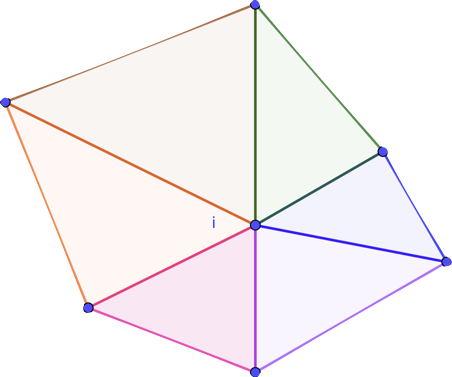
\includegraphics[width=0.8\linewidth]{figures/unit_area}
			  \captionof{figure}{Areas of one-ring triangles}
			  \label{fig:unit-area}
		\end{minipage}%
		\begin{minipage}[t]{.55\textwidth}
			  \centering
			  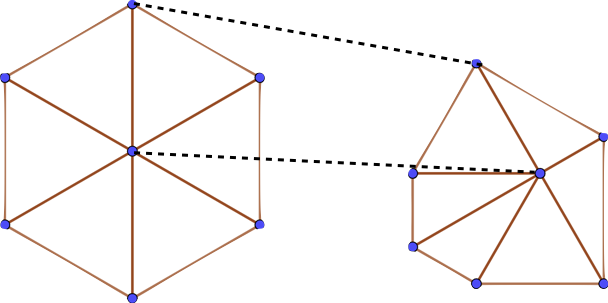
\includegraphics[width=0.9\linewidth]{figures/arap}
			  \captionof{figure}{ARAP defined with “spokes and rims” edges }
			  \label{fig:arap}
		\end{minipage}
	\end{figure}
%-------------------------------------------------------------------
% ARAP
%-------------------------------------------------------------------
\subsubsection{As-Rigid-As-Possible}\label{arap}
As-Rigid-As-Possible Surface Modeling \cite{arap} is a method to address this issue. This is a work from Sorkine and Alexa in year 2007, and it's cited and used by lots of different papers. 
	\begin{equation}
		ARAP:=\sum_{i\in V}\sum_{j\in N(i)} \left\lVert R_i d_{i,j} - \tilde{d}_{i,j} \right\rVert _F^2
		\label{eq:arap}
	\end{equation}
Here, the formula \ref{eq:arap} enforces the edges of deformed state $\tilde{d}_{i,j}$ is identical to the original state $d_{i,j}$ up to a rigid transformation (here means rotation $R_i$). $N(i)$ is the “spokes and rims” edges, see figure \ref{fig:arap}.\\

Once we have defined the cubeness term and ARAP term, the objective function is within reach. 
\begin{equation}
	\underset{\tilde{V},R_i}{\min} = \sum_{i\in V}\sum_{j\in N(i)} \frac{w_{i,j}}{2}\left\lVert R_i d_{i,j} - \tilde{d}_{i,j} \right\rVert _F^2 +  \lambda a_i\left\lVert R_i \hat{n}_i\right\rVert _1
	\label{eq:obj}
\end{equation}

As all kinds of optimization problems, when putting two different terms together, usually additional parameters are added in front of at least one of them to control the weights, and each term is emphasized by the value of the weights. The authors \cite{Liu:CubicStyle:2019} add three, $w_{i,j}$ in front of ARAP term, and $\lambda$ and $a$ in front of cubeness term. $w_{i,j}$ represents the cotangent weight, it is the sum of cotangent of angles opposite of edge $(i,j)$, the edge shared by two triangles, see in figure \ref{fig:cot}. $a$ is barycentric area, the area of the region bound by barycenters of neighboring triangles, figure \ref{fig:bary}. $\lambda$ is a totally free parameter for user to control the deformation. More will be discussed in section \ref{artistic}.
	\begin{figure}[ht!]
		\centering
		\begin{minipage}[t]{.45\textwidth}
			  \centering
			  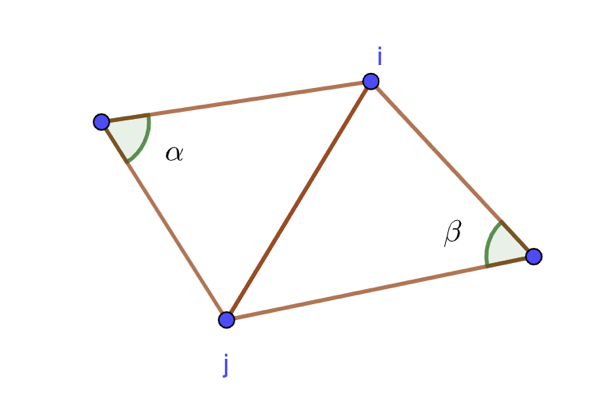
\includegraphics[width=0.95\linewidth]{figures/cot}
			  \caption{Cotangent weight defined around the edge $(i,j)$}
			  \label{fig:cot}
		\end{minipage}%
		\begin{minipage}[t]{.45\textwidth}
			  \centering
			  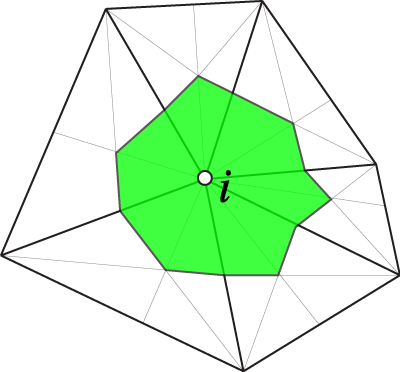
\includegraphics[width=0.7\linewidth]{figures/barycentric}
			  \caption{Barycentric area at vertex $i$}
			  \label{fig:bary}
		\end{minipage}
	\end{figure}

Specifically, cotangent weights are used for mitigating the problem caused by meshing bias during deformation \cite{arap}. Barycentric area enforces large cubeness on vertices surrounded by large triangles, and let small triangles to preserve the local detail.

%-----------------------------------------------------------------------------------------------------
% Optimization
%-----------------------------------------------------------------------------------------------------
\subsection{Optimization}\label{opt}

Once we get the objective function, the next question to answer is how to solve it. The Cubic Stylization paper follows the ARAP paper, and uses the local-global scheme. They proposed that first calculate the rigid body transformation locally, then update the vertices in a global manner. As the rigid body transformation only holds locally. If it holds for entire mesh, then the deformation will collapse to a rotation which has no stylization effects. \\

Let's have a look at the local step, local in the sense of ``spokes and rims" region. Firstly, the objective is re-written as follows.
	\begin{equation}
		R_i^{\star} = \underset{R_i \in SO(3)}{\arg \min}\frac{W_{i}}{2}\left\lVert R_i D_i - \tilde{D}_i \right\rVert _F^2 +  \lambda a_i\left\lVert R_i \hat{n}_i\right\rVert _1
	\label{eq:local}
	\end{equation}
Then the author reformulate the function:
	\begin{equation}
		\underset{z, R_i \in SO(3)}{minimize} \quad \frac{W_{i}}{2}\left\lVert R_i D_i - \tilde{D}_i \right\rVert _F^2 +  \lambda a_i\left\lVert z\right\rVert _1
		\quad \quad
		s.t. \quad z-R_i \hat{n}_i = 0
		\label{eq:reformulate}
	\end{equation}

The advantage of doing this is that they can use the method call Alternating Direction Methods of Multipliers. 

%-------------------------------------------------------------------
% ADMM
%-------------------------------------------------------------------
\subsubsection{Alternating Direction Method of Multipliers}\label{admm}
Alternating Direction Method of Multipliers, or abbreviated as ADMM \cite{admm}, is an algorithm that solves convex optimization problems by breaking them into smaller pieces, each of which are then easier to handle. It is a variant of the standard augmented Lagrangian method. The later is formulated as minimizing a function with constraints, \[\min f(x) \quad s.t. \quad c_{i\in I}(x) = 0.\] The update rule for $k$-th iteration is 
	\begin{equation}
		\begin{split}
		\min \Phi_k(x) &= \min f(x) + \sum_{i\in I}\beta_ic_i(x) + \frac{\rho_k}{2}\sum_{i\in I}c_i(x)^2\\
		\beta_{k+1} &\leftarrow \beta_k + \rho_k c_i(x_k)
		\end{split}
		\label{eq:update}
	\end{equation}

ADMM alters the problem with a trick. If the object function is linear separable, then it replace the second chuck with a different parameter, and add a constraint like equation \ref{eq:reformulate}.
\[\min f(x)+g(x) \iff \min f(x)+g(y) \quad s.t. \quad x=y.\]

Following update rules \ref{eq:update}, the update rule for ADMM can be derived as
	\begin{equation}
		\begin{split}
			\min \Phi_k(x) &= \min f(x) + g(y) + \beta(x-y) + \frac{\rho_k}{2}(x-y)^2 \\
				&= \min f(x) + \beta x + \frac{\rho_k}{2}(x-y)^2 \\
				&= \min f(x) + \frac{\rho_k}{2}(x-y + u)^2 + const,\\
			\min \Phi_k(y) &= \min f(x) + g(y) + \beta(x-y) + \frac{\rho_k}{2}(x-y)^2 \\
				&= \min g(y) + \frac{\rho_k}{2}(x_{k+1}-y + u)^2 + const,\\
				u_{k+1} &\leftarrow u_k + x_{k+1} - y_{k+1}
		\end{split}
		\label{eq:admm_org}
	\end{equation}

Given our optimization problem \ref{eq:local}, the update rules can be derived by substituting equations \ref{eq:admm_org} piece by piece
	\begin{equation}
		\begin{split}
			R_i^k &\leftarrow \underset{R_i\in SO(3)}{\arg \min} \frac{W_{i}}{2}\left\lVert R_i D_i - \tilde{D}_i \right\rVert _F^2 +  \frac{\rho^k}{2} \left\lVert R_i\tilde{n}_i - z + u^k\right\rVert _2^2\\
			z^{k+1} &\leftarrow \underset{z}{\arg \min} \lambda a_i\left\lVert z\right\rVert _1 + \frac{\rho^k}{2} \left\lVert R_i^{k+1}\tilde{n}_i - z + u^k\right\rVert _2^2\\
			\tilde{u}^{k+1} &\leftarrow u^k + R_i^{k+1}\tilde{n}_i - z^{k+1}\\
			\rho^{k+1}, u^{k+1} &\leftarrow update(\rho^k)
		\end{split}
	\end{equation}
	
The step of updating $R$ is called orthogonal Procrustes \cite{Procrustes}; $z$ is calculated as LASSO problem using shrinkage step \cite{admm}.\\

After run the ADMM for solving the optimization problem, we finally get $R$ for every vertex. As we discussed in the beginning of this section, we need a global step to update the positions of vertices. This is done by find the solution of a linear equation system. 
	\begin{equation}
		\sum_{j\in N(i)} w_{i,j} \tilde{d}_{i,j} =\sum_{j\in N(i)} \frac{w_{i,j}}{2}(R_i+R_j)d_{i.j}
	\end{equation}
We want the positions of edge of deformed state $\tilde{d}_{i,j}$ to agree on all neighboors' rigid body transformations calculated in local step to an extent.

%-------------------------------------------------------------------
% Affine
%-------------------------------------------------------------------
\subsubsection{Affine Progressive Mesh}\label{affine}
As sometimes the sophisticated meshes contains millions of face, see figure \ref{fig:faces}, thus, the author also adapts a method called Affine Progressive Mesh into the process. This is a work published by Manson and Schafer in year 2011 \cite{affine}. It aims to address the runtime problem on high resolution meshes. \\

The core idea is to downsample the total vertices, take note of sequence of vertices merges, after some other time consuming operations, then expand them back by fitting best affine transformation, shown in figure \ref{fig:merge}. For high degree of cubeness, the local rigidity is hard to hold. So we loose the constraint by substituting the rigid transformation to an affine transformation.
	\begin{figure}[ht!]
		\centering
		\begin{minipage}[t]{.3\textwidth}
			  \centering
			  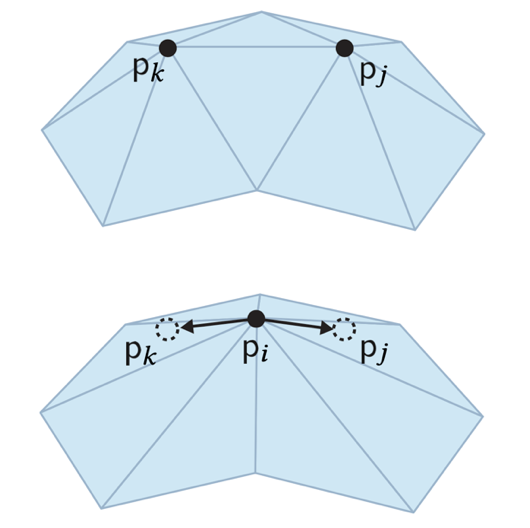
\includegraphics[width=\linewidth]{figures/merge_split}
			  \caption{Edge collapses}
			  \label{fig:merge}
		\end{minipage}%
		\begin{minipage}[t]{.65\textwidth}
			  \centering
			  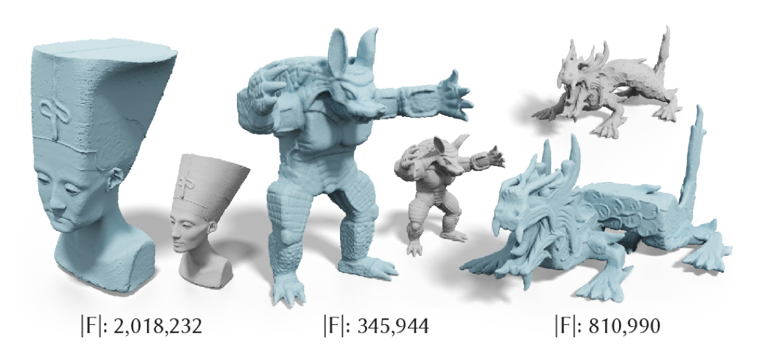
\includegraphics[width=0.9\linewidth]{figures/face}
			  \caption{Numbers of faces of different meshes}
			  \label{fig:faces}
		\end{minipage}
	\end{figure}

Note that this worked as a pre-processing step before cubic stylization, which means the cubic stylization runs on the coarsest mesh after edge collapsing. After deformation, the vertices are split again to visualize the final result on the original resolution. The reason to emphasis this is that according to the authors, the runtime is measured only for cubic stylization, not the whole downsampling to upsampling steps, which is typically several times longer than the stylization.

%-----------------------------------------------------------------------------------------------------
% Artistic constrols
%-----------------------------------------------------------------------------------------------------
\section{Artistic Controls}\label{artistic}
	\begin{figure}[hbt!]
		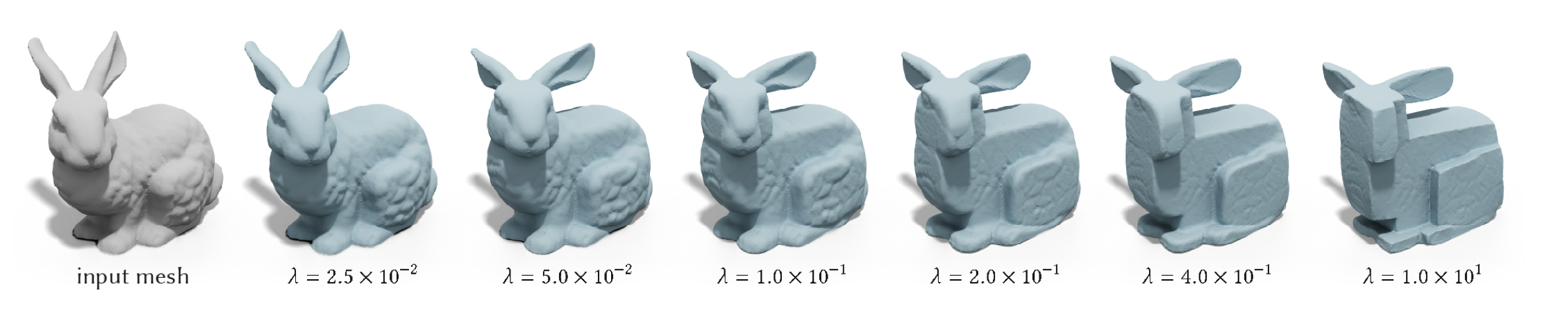
\includegraphics[width=\linewidth]{figures/lambda1}
		\caption{Control the cubeness through changing the value of $\lambda$}
		\label{fig:lbd1}
	\end{figure}

Given the objective function \ref{eq:obj} let's have a look of what kind of artistic controls are provided by the model. As $\lambda$ is the parameters before the cubeness term, therefore, a large lambda stands for higher emphasis on cubeness, see in figure \ref{fig:lbd1}. We can also split the single $\lambda$ into a set of parameters. For example, 3, and each of them takes care of the cubeness in one direction of the global coordinate. Check the illustration on the left part of the figure \ref{fig:lbd4}. This can go further by generating a gauss map with continuous changing value for $\lambda$, and mapped onto the mesh. Different parts have different degrees of cubeness.
	\begin{figure}[ht!]
		\centering
		\begin{minipage}[t]{.45\textwidth}
			  \centering
			  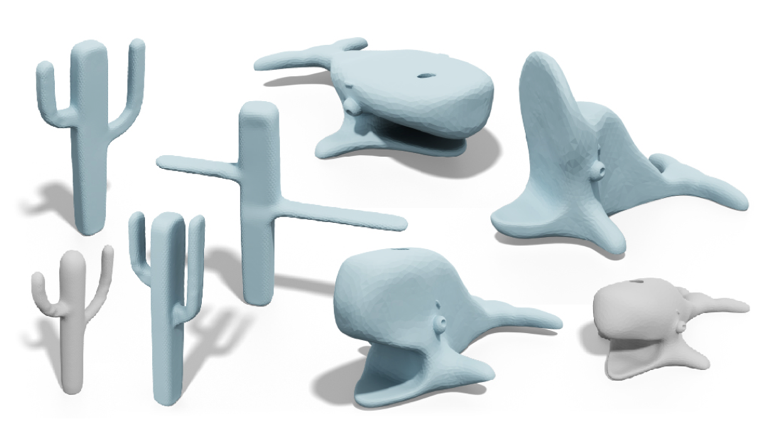
\includegraphics[width=\linewidth]{figures/lambda2}
			  \label{fig:lbd2}
		\end{minipage}%
		\begin{minipage}[t]{.55\textwidth}
			  \centering
			  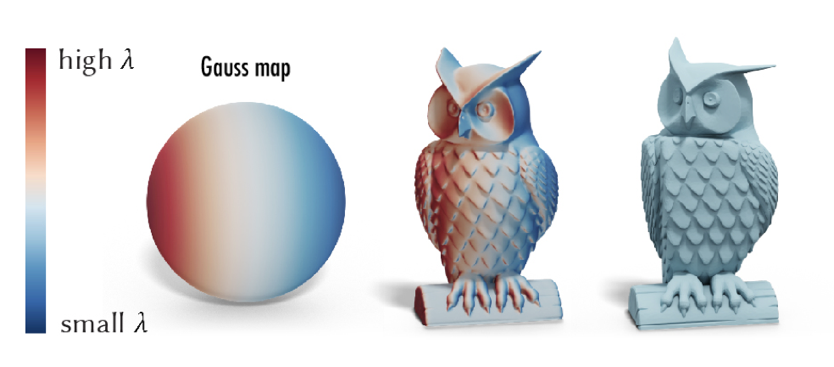
\includegraphics[width=0.9\linewidth]{figures/lambda3}
			  \label{fig:lbd3}
		\end{minipage}
		\caption{Control the cubeness through changing the value of $\lambda_d$ (for $d\in\{1,2,...,n\}$)}
		\label{fig:lbd4}
	\end{figure}
Moreover, a modeler can insert several local coordinate systems into the $\ell$1-norm, and create a polyhedric stylization, no matter uniform or non-uniform cube orientations, see figure \ref{fig:poly}.
	\begin{figure}[hbt!]
		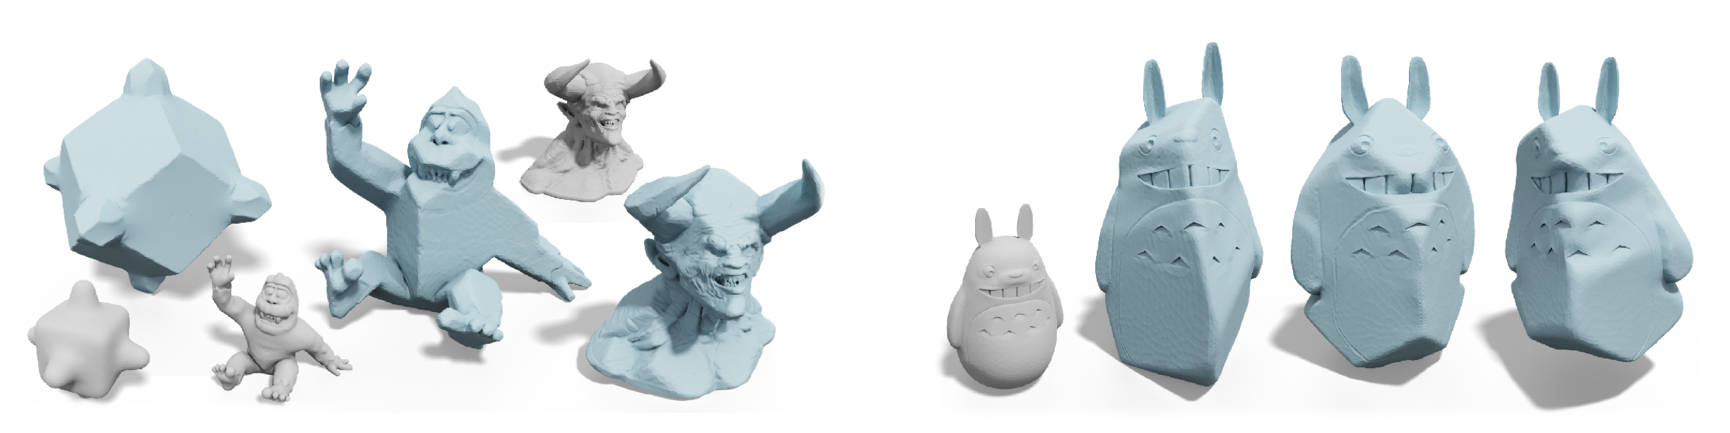
\includegraphics[width=\linewidth]{figures/coordinate}
		\caption{Apply a coordinate transformation inside $\ell$1-norm to generalize cubic stylization to polyhedrons.}
		\label{fig:poly}
	\end{figure}


%-----------------------------------------------------------------------------------------------------
% Summary
%-----------------------------------------------------------------------------------------------------
\section{Summary }\label{sum}
In general, this is an interesting work which draws a link between art and sciences. It creates a clear stated mathematical tool for cubic stylization while provides some free controls at the same time. The mainly downside still remains at computational time, which barely reaches on-the-fly performance with a commodity hardware setup. Nevertheless, this work shoots a beam of light to model more intricate styles.

\newpage
\bibliographystyle{plain}
\bibliography{report}



\end{document}